%% Using-the-MC-LaTeX-Class.tex
%
% Copyright (C) 2008-2010 Fabrice Niessen
% Time-stamp: <2010-01-13 Wed 12:19 sva on mundaneum>
%
\listfiles
\documentclass{mcreport}
\usepackage[utf8]{inputenc}
% \DeclareUnicodeCharater{00A0}{ } % pdftex en utf8
\usepackage{tikz}
\usetikzlibrary{backgrounds}

\usepackage{movie15} % for inserting avi multimedia files
\usepackage{multido}

\usepackage{datatool}
\DTLloaddb{nmap-audit}{csv-report.csv}

\title{Using the MC \LaTeX{} Class}
\hypersetup{
    pdfsubject={LaTeX class},
    pdfkeywords={mc reports latex class}}
\author{Fabrice Niessen \\ \href{mailto:fni@missioncriticalit.com}{fni@missioncriticalit.com}}
\date{\today}

\hfuzz=10000pt % dans l'exemple, je ne veux pas de message sur les
% Overfull hbox.

\tracingpages=1
\tracingonline=1 % si on ne veut pas regarder dans le fichier log

\hyphenation{mis-sion-cri-ti-cal-it er-go-no-mic}
% Don't use the comma. The space separates the words.



\begin{document} %------------------------------------------------------------
\selectlanguage{english}
% \mtcselectlanguage{english} % for minitoc

\maketitle[caption=Internal documentation]

\newpage


\tableofcontents

\mccomment[fni]{The section headings are linkable.}

\mccomment[fni]{BTW, this is a comment provided by the `mcreport' class.}

\newpage


\section{Context}
\label{sec:context}

In this document, I will describe how to use the \acs{MC} class,
\mccomment[fni]{The acronym is an hyperlink as well.} and I will show
different features you can use within \LaTeX{}. This way, you can easily
figure out how to do things you see implemented here --- a sort of huge
reference card...

But, first, some other topics.

\subsection*{Why Using \LaTeX{}?}
\label{sec:why-choosing-latex}

\begin{itemize}
    \item It's free.

    \item It's portable.

    \item Its output quality\footnote{Kerning, real small caps, ligatures,
    hyphenation, etc.} is far superior to other word processing products ---
    see, for example, how the beginning of the
    ``V'' is positionned before the end of the ``A'' in ``AVANT'': \\
    {\fontsize{40pt}{30pt}\selectfont AVANT},
    {\fontsize{40pt}{30pt}\selectfont ~Table},
    {\fontsize{40pt}{30pt}\selectfont ~fire}. \\
    Type the same words in other word processors, in big fonts, and you will
    be surprised how it looks like.

    \item You can structure the whole document with very few mark-ups
    (lightweight language intended for human consumption).

    \item There are tons of packages (more than 2,687) to allow you to do
    whatever you've ever dreamed of. Have a look at \acs{CTAN}
    (\url{http://www.ctan.org/search.html}).
    \mccomment[fni]{Link is broken on 2 lines, but still clickable.}

    \begin{figure}[!ht]
        \centering
        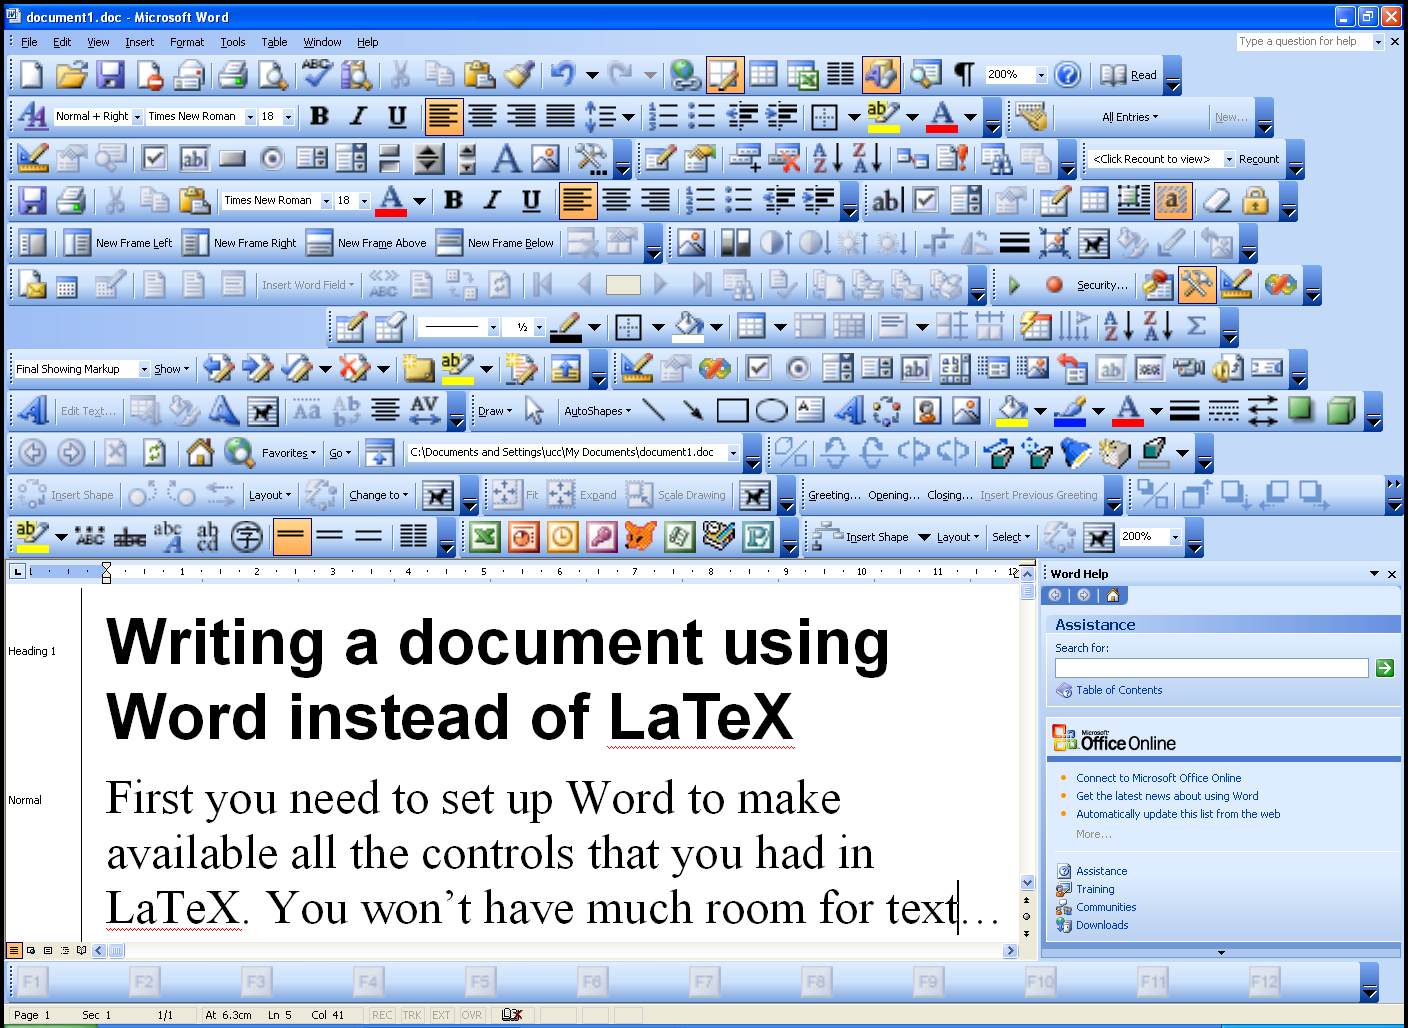
\includegraphics[width=11cm]{images/MS-Word-competition}
        \caption{Microsoft Word as competition for LaTeX}
        \label{fig:logo-mc}
    \end{figure}

    \item It is \acs{WYSIWYM}.

    \item You can even write good-looking slides with the \texttt{beamer}
    package.
\end{itemize}


\section{The MC Class}
\label{sec:mc-class}

How to use the MC class?  Easy... Just replace:

\begin{verbatim}
\documentclass{article}
\end{verbatim}

by:

\begin{verbatim}
\documentclass{mcreport}
\end{verbatim}

That should do the trick, if \url{mcreport.cls} is in your \acs{TDS} (\TeX{}
Directory Structure --- where all the other packages are located), probably
to be found at \url{~/texmf/tex/latex/}.

Eventually, run \url{texhash} or update FNDB (MiKTeX) so that \LaTeX{} can
update its directory structure for references, and you'll be good to go.

\subsection{Options}
\label{sec:options}

Options are basically order-independent.

The \texttt{mcreport} class currently accepts three mutually exclusive
\mcobj{options}:

\begin{itemize}
    \item \textbf{article} --- used to indicate short documents based on the
    \textsf{article} class(this is the default);
    \item \textbf{report} --- used to indicate longer documents based on the
    \textsf{report} class;
    \item \textbf{book} --- used to indicate long documents based on the
    \textsf{book} class.
\end{itemize}

The impact of choosing one over the other is that, in \emph{report} or
\emph{book} documents:

\begin{itemize}
    \item chapters are supported (even mandatory); in \emph{article} ones,
    they are not.
    \item minitoc are available (wherever you insert the \verb|\minitoc|
    macro).
\end{itemize}

As well, it accepts the options:

\begin{itemize}
    \item \textbf{final} for removing all \textit{draft marks} (which are put
    \emph{by default}),
    \item \textbf{black} for removing all colors from the titles and the
    hyperlinks.
\end{itemize}

\subsection{New Macros}
\label{sec:macros}

\begin{itemize}
    \item mccomment --- note in the left margin (``à la Microsoft''
    reviewing comments). It takes 2 arguments: (optionally) the initials of
    the author, and (mandatory) the note
    itself. \\
    \verb|\mccomment[fni]{This is a comment.}|
\end{itemize}

\subsection{New Environments}
\label{sec:environments}

\begin{itemize}
    \item mcnote --- sort of intermezzo. \\
    \verb|\begin{mcnote} This is a note. \end{mcnote}|
\end{itemize}

% \subsection{Code of the Class}
% \label{sec:code-class}
% 
% \lstinputlisting
% [language=TeX,%
% caption=Code of the MC class,%
% label=lst:this-doc]
% {mcreport.cls}


\section{Tools}
\label{sec:tools}

\href{http://code.google.com/p/latexdaemon/}{LaTeXdaemon} and
\href{http://blog.kowalczyk.info/software/sumatrapdf/}{Sumatra PDF} provide
a very nice ``almost real time translation and viewing''.

Emacs + AUCTeX +
\href{http://www.gnu.org/software/auctex/preview-latex.html}{preview-LaTeX}
also provide \acs{WYSIWYG} previewing.


\section{Note}
\label{sec:note}

La commande \verb|\\| sert à passer à la ligne DONC :

\begin{itemize}
    \item ne sert pas à changer de paragraphe (ou d'alinéa) en supprimant
    (momentanément) le retrait d'alinéa ; pour cela, on a \verb|\noindent|
    ou \verb|\setlength{\parindent}{0pt}| ;

    \item ne sert pas à augmenter l'espacement vertical entre deux
    paragraphes (alinéas) ; pour cela, on a \verb|\par\vspace{<dimension>}|.
\end{itemize}

J'ajouterai que pour aérer entre les paragraphes on a aussi
\verb|\smallskip|, \verb|\medskip| et \verb|\bigskip|, ce qui permet souvent
d'être plus cohérent qu'en mettant des \verb|\vspace| si on n'y fait pas
gaffe.

De façon positive, \verb|\\| ne devrait faire bondir personne lorsqu'on
cherche, par exemple, à :

\begin{itemize}
    \item écrire les vers d'une poésie (encore que je verrais plutôt une
    redéfinition locale du saut de ligne pour remplacer \verb|\\|) ;

    \item écrire des blocs du type
    Jean-Côme Charpentier\verb|\\|
    3,1415 rue Pyth\verb|\\|
    31415 MONZAC 5e

    \item passer à la ligne dans un tableau mais c'est limite triche parce
    que LaTeX modifie la définition de \verb|\\| lorsqu'on se trouve dans un
    environnement tabular ou apparenté.
\end{itemize}

Une remarque générale en passant : il faut prendre garde à toujours mettre
un \verb|\par| avant le \verb|\vspace| sauf si on veut vraiment obtenir des
effets spéciaux : le \verb|\vspace| tout seul ne met pas fin au pragraphe
courant.


\section{Interesting Packages}
\label{sec:interesting-packages}

\subsection{Coding System}
\label{sec:coding-system}

To support accents encoded in UTF-8, add this to your preamble:

\begin{verbatim}
\usepackage[utf8]{inputenc} % or latin1
\end{verbatim}

\subsection{Typography}
\label{sec:typography}

\begin{itemize}
    \item babel --- makes all what's needed for cesure, typography, plus
    some macros (for 1\ier, 2\ieme, \no, \degres centigrades), etc..
    \item french (commande sommaire)
    \item minitoc
    \item lettrine
\end{itemize}

You need pdftex 1.40.4 to have ligatures in letterspaced text.

\textls[35]{--- my text <<}

\subsection{Layout}
\label{sec:layout}

\begin{itemize}
    \item fancyhdr
    \item geometry
\end{itemize}

\subsection{Links}
\label{sec:links}

\subsubsection{hyperref}
\label{sec:hyperref}

\href{http://www.google.com}{This text} is an hyperlink which will be
resolved into the URL of Google.

\verb|\autoref| is a substitution for the standard \verb|\ref| command. It
inserts a context sensitive label, like \autoref{sec:links}.

\subsubsection{url}
\label{sec:url}

This new defined command \verb|\urlw| allows the user to typeset a linkable
(this function is offered by \href) and breakable address like this:

\url{http://www.hackaday.com/2008/08/06/black-hat-2008-fastrak-toll-system-completely-broken/}

\url{http://www.nowhere.com/xxVERY/xxxLONG/xxxxxURL/xxxxxxWITH/xxxxxxMANY/xxxxxSLASHES/xxxxIN/xxxIT}

% \url{http://www.thelongestlistofthelongeststuffatthelongestdomainnameatlonglast.com/wearejustdoingthistobestupidnowsincethiscangoonforeverandeverandeverbutitstilllookskindaneatinthebrowsereventhoughitsabigwasteoftimeandenergyandhasnorealpointbutwehadtodoitanyways.html}

% \urlw{http://www.thelongestlistofthelongeststuffatthelongestdomainnameatlonglast.com/wearejustdoingthistobestupidnowsincethiscangoonforeverandeverandeverbutitstilllookskindaneatinthebrowsereventhoughitsabigwasteoftimeandenergyandhasnorealpointbutwehadtodoitanyways.html}

\subsection{Verbatim}
\label{sec:verbatim}

\subsubsection{verbatim Package}
\label{sec:verbatim-package}

\begin{verbatim}
This is verbatim
LaTeX is funny!
\end{verbatim}

\subsubsection{listings Package}
\label{sec:listings-package}

But there is more: you can insert snippets of code which will be
automatically highlighted in the appropriate color (thus, depending on the
programming language used in the snippet).

You don't believe me?  Here follows a proof:

\lstset{language=C}
\begin{lstlisting}
// put your code here
if (var == 1)
    for (i = 1; i < 10; i++)
        printf(atoi(i));
else
    str = "my string";
\end{lstlisting}

\subsubsection{Underline}

You can't write \verb|\ul{a text with \ref{section}}|, but it is still
possible to use \verb|\ref| inside \verb|\ul|:
\ul{a text with \mbox{\autoref{sec:interesting-packages}}}

\subsection{Graphics and colors}
\label{sec:graphics-colors}

\subsubsection{graphics Package}

When inserting graphics, don't put an extension to the filename... See the
example of \autoref{fig:logo-mc}.

\begin{figure}[!ht]
    \centering
    
\includegraphics[width=2cm]{images/MissionCriticalIT}
    \caption{Include PNG graphic}
    \label{fig:logo-mc}
\end{figure}

If you're using what's know as "pdfLaTeX", know it only accepts graphics in
(bitmap) PNG, JPG, or (scalable) PDF form.

\begin{mcnote}
    For including vector drawings, it's better to furnish them directly in
    the PDF format.
    Though, EPS should be usable with the package purifyeps (not tested).
\end{mcnote}

\subsubsection{TikZ/PGF Package}

In the same spirit as the \acs{SVG} now does, you can also ``program''
graphics with ``TikZ and PGF'', as the following example of code shows it:

\begin{verbatim}
\begin{tikzpicture}
    \begin{scope}[xshift=0.5cm,yshift=0.5cm]  % moving a group of nodes
        \draw[very thick, color=red, rounded corners=8pt]
        (0,0) -- (0,2) -- (1,3.25) -- (2,2) -- (2,0) -- (0,2) -- (2,2)
        -- (0,0) -- (2,0);
    \end{scope}
    \draw[draw=red!10]
        (0,0) grid[step=.2] (current bounding box.north east);
    \draw[draw=gray!30]
        (current bounding box.south west) grid
        (current bounding box.north east);
\end{tikzpicture}
\end{verbatim}

which gives:

\begin{tikzpicture}
    \begin{scope}[xshift=0.5cm,yshift=0.5cm]  % moving a group of nodes
        \draw[very thick, color=red, rounded corners=8pt] (0,0) -- (0,2) --
        (1,3.25) -- (2,2) -- (2,0) -- (0,2) -- (2,2) -- (0,0) -- (2,0);
    \end{scope}
    \begin{pgfonlayer}{background}
    \draw[draw=red!10] (0,0) grid[step=.2] (current bounding box.north east);
    \draw[draw=gray!30] (current bounding box.south west) grid
                        (current bounding box.north east);
    \end{pgfonlayer}
\end{tikzpicture}

Doing so, you get all the advantages of the ``\TeX-approach to
typesetting'':

\begin{itemize}
    \item quick creation of simple graphics,
    \item precise positioning,
    \item the use of macros,
    \item often superior typography,
    \item and the \emph{text in the graphics in the same size as the text of
    the document} (whichever scaling factor you apply afterward).
\end{itemize}

Plus the possibility to make references between the text and the graphics
(having, for example, a graphics with ``see section 2'' in some label).

You also inherit all the disadvantages: steep learning curve, no
\acs{WYSIWYG}, small changes require a long recompilation time, and the code
does not really ``show'' how things will look like.

But, with TikZ, you can support \emph{properties that aren't supported by
GUI drawing applications} like CorelDRAW:

\begin{itemize}
    \item linking nodes by arrows so they are oriented from node center to
    node center (rather that from/to predetermined "connection points") with
    the edges shadowed exactly as needed by the node shape (look at
    \href{http://www.cs.queensu.ca/students/undergraduate/prerequisites}
    {http://www.cs.queensu.ca/students/undergraduate/prerequisites});

    \item drawing nodes that exactly enclose the contained text (with a
    standard spacing).
\end{itemize}

\subsubsection{xcolor Package}

\verb|\color{red}| puts some text \color{red}{in red}\color{black}.

\subsubsection{fancybox}

Oval boxes

\subsubsection{wrapfig}

Make a figure float inside a paragraph

\subsubsection{psfrag}

% \begin{figure}[ht]
%     \includemovie[
%     poster,
%     text={\small(Click to start M2U01777.mpg)}
%     ]{.5\linewidth}{.375\linewidth}{M2U01777.mpg}
% \end{figure}

% \usepackage[final]{movie15}
% \includemovie[
% autoplay, autopause,
% inline=true,
% controls=false,
% repeat=5,
% poster,
% playerid=MSFT_WindowsMediaPlayer, % Désolé
% rate=1,
% text={\small(Please wait while hopefully loading movie\ldots)}
% ]{1\textwidth}{0.8\textheight}{rotation.avi}

À ma connaissance, sous Linux, aucun viewer PDF ne permet de jouer une vidéo
directement intégrée dans la vue PDF. Par contre, certains savent lancer un
viewer externe (donc dans une fenêtre séparée).

Avec 'acroread' ou 'evince' :

Via beamer et sa commande \verb|\movie| avec l'option 'externalviewer', on
peut lancer une vidéo. Le nom du fichier à fournir est celui de la vidéo.
Pour choisir le viewer externe, acroread ou evince se réfère au réglage du
gestionnaire de fichiers : nautilus pour gnome, konqueror pour KDE ou thunar
pour xfce. Défaut : il ne me semble pas possible de spécifier les options à
passer au viewer.

Avec 'xpdf' :

Toujours via beamer et sa commande \verb|\movie| avec l'option
'externalviewer', on peut lancer une vidéo. Par contre, il faut lui indiquer
le chemin *absolu* d'un script qui s'occupera de lancer un viewer avec la
bonne vidéo. Ce passage par un script externe permet de choisir le viewer et
surtout les options qu'on veut pour chaque vidéo (par exemple, une vue en
plein écran). Par contre, je n'ai pas trouvé comment l'empêcher de demander
une confirmation à chaque lancement d'une vidéo. Autre défaut mais mineur :
le lancement de la vidéo depuis le PDF n'est pas compatible Windows ou MacOS
X.

Dans tous les cas, il faudra créer soi-même l'image de présentation
cliquable qui apparaîtra à l'emplacement prévu dans le fichier PDF.


\subsection{Mathematical mode}
\label{sec:mathematical-mode}

amsmath --- Text in mathematical mode, matrix, multi-line formulas

You can very easily insert (numbered) mathematical equations in your
document, such as:

\begin{equation}
    \label{eq:1}
    L = \frac{\pi^2 10^{-7} N^2 A^2}{B}
\end{equation}

for computing the inductance of a solenoid.

\subsection{Symbols}
\label{sec:symbols}

\subsubsection{eurosym Package}
\label{sec:eurosym-package}

According to the (first) official rules, the euro symbol has always to
remain ``sans serif'':

\begin{itemize}
    \item this costs 10 \euro;
    \item \textsf{this costs 10 \euro;}
    \item \texttt{this costs 10 \euro;}
\end{itemize}

\mccomment[FNI]{Check that the symbol is displayed in your font.}
but changes to bold and/or italic as needed:

\begin{itemize}
    \item this costs 10 \euro;
    \item \textbf{this costs 10 \euro;}
    \item \textit{this costs 10 \euro;}
    \item \textit{\textbf{this costs 10 \euro;}}
\end{itemize}

\subsubsection{latexsym}

Symbols

\subsubsection{amssymb}

Symbols (triangle)

\subsubsection{pifont}

\texttt{pifont} is for Zapfs Dingbats. For example, a number in a circle is
to be found there.

\subsection{Tables}
\label{sec:tables}

\begin{tabular}{|l|p{4cm}|} \hline
    Topic 1 & Topic 2 \\
    \hline
    Some long long long long long long long long long long long text &
    More long long long long long long long long long long text, broken onto
    several lines\\
    \hline
\end{tabular}

Use the columntype p{<width>} instead of "l", to automatically add line
breaks.

\subsubsection{tabular Package}
\label{sec:tabular-package}

The basic environment for tables in \LaTeX{} is \texttt{tabular}. It creates
a table whose width is automatically set, based on the content.

\begin{table}[!ht]
    \centering
%     \rowcolors{1}{RoyalBlue!20}{RoyalBlue!5}
    \begin{tabular}{| c | p{2cm} | r |}
        \hline
        centered     & \multicolumn{2}{c|}{left-aligned and right-aligned} \\
        \hline
        1.1          & 1.2                & 1.3                            \\
        \cline{2-3}  & 2.2                & 2.3                            \\
        \hline
        3.1          & 3.2                & 3.3                            \\
        \hline
    \end{tabular}
    \caption{Table with merged lines and columns}
    \label{tab:table}
\end{table}

The total width of the table can only be defined with \verb|tabular*|.

\subsubsection{array Package}
\label{sec:array-package}

But, even if we don't need specific functionality, it is useful to declare
the \texttt{array} package, which fixes a certain number of defaults, and
brings some fantasy with the tables.

\begin{mcnote}
    Attention: the \texttt{array} \emph{environment} is for mathematical
    tables. Do not confuse...

    En fait, il y a peu de cas où on a vraiment besoin de array de nos jours
    (voir aligned, cases, matrix, pmatrix, etc d'amsmath).
\end{mcnote}

\subsubsection{booktabs Package}
\label{sec:booktabs-package}

The booktabs package allows for publishing quality tables in \LaTeX{}.

Two of their advised guidelines are:

\begin{itemize}
    \item Never, ever use vertical rules.
    \item Never use double rules.
\end{itemize}

\begin{table}[!ht]
    \centering
    \begin{tabular}{@{}llr@{}} \toprule
        \multicolumn{2}{c}{Item} \\ \cmidrule(r){1-2}
        Animal & Description & Price (\$)\\ \midrule
        Gnat & per gram & 13.65 \\
        & each
        & 0.01 \\
        Gnu
        & stuffed
        & 92.50 \\
        Emu
        & stuffed
        & 33.33 \\
        Armadillo & frozen & 8.99 \\ \bottomrule
    \end{tabular}
\end{table}

(Get example of \url{http://www.tug.org/pracjourn/2007-1/mori/mori.pdf})


% \newcolumntype{L}{>{\raggedright\arraybackslash}p}
% \begin{table}[hbtp]
%     \caption{Description of steps involved in research methodology}
%     \centering
%     % Table generated by Excel2LaTeX from sheet 'Sheet1'
%     \begin{tabular}{L{0.5cm}L{2cm}L{2.5cm}L{3.5cm}L{3.5cm}}
%         \toprule
%         Step  & Theme &  Objective & Overall Research Question &
%         Process \\
%         \midrule
%         1 & Data Preparation &  To collect dataset of experiment &
%         What types of dataset best represent the language identification
%         problem, how to collect it and how to overcome diverse character sets
%         issue? & Requirement analysis, data collection, data selection and
%         data integration \\
%         \midrule
%         2 & Data Preprocessing & To implement the data preprocessing
%         method & What is problem of collected dataset and how to do data
%         preprocessing? & Data inspection and data processing \\
%         \midrule
%         3 & Feature Selection & To find out most relevant features &
%         What types of features best represent the samples have been collected
%         and how to improve feature selection method? & Entropy, Letter
%         Weighting and Simplified Entropy \\
%         \midrule
%         4 & Identification & To determine the predefined language
%         automatically & How to do language identification? & Fuzzy ARTMAP and
%         Rule Based Decision \\
%         \bottomrule
%     \end{tabular}
%     \label{infoReMe}
% \end{table}




\subsubsection{datatool Package}

datatool has macros to open a \path{.csv} file, process it, and close it.

\begin{table}[!ht]
    \centering
    {
    \fontsize{9pt}{11pt}\selectfont
    \begin{tabular}{rlccrcl}
        NUM & HOSTNAME & IP & STATE & PORT & PROTOCOL & SERVICE
        \DTLforeach{nmap-audit}{\hostname=HOSTNAME, \ip=IP, \state=STATE,
        \port=PORT, \protocol=PROTOCOL, \service=SERVICE}{%
            \DTLiffirstrow{\\\hline}{\\}
            \theDTLrowi.&\hostname&\ip&\state&\port&\protocol&\service}
    \end{tabular}
    }
\end{table}

\subsubsection{Automatic generation of tables}
\label{sec:autom-gener-tabl}

Finally, if you use Microsoft Excel, there is a small free plug-in, called
\texttt{excel2latex}, that will let you create your tables in Excel and
export them to \LaTeX{}.

\subsection{Fonts}
\label{sec:fonts}

We can use fonts in whichever size, as shown here (from 1 pt to 32 pt):

\multido{\i=1+1}{32}{\fontsize{\i}{\i}\selectfont A}

% you can change the values to see other fonts
\mcshowfont{T1}{cmr}{m}{n}
\mcshowfont{T1}{phv}{m}{sc}
\mcshowfont{T1}{ptm}{b}{it}
\mcshowfont{U}{pzd}{m}{n}

Si tu veux utiliser une fonte de façon ponctuelle, tu peux utiliser

\begin{verbatim}
{\fontfamily{<nom>}\selectfont le texte dans cette fonte}
\end{verbatim}

La seule difficulté est de trouver le <nom> à utiliser. Pour ça, en général
je lis rapidement le code du paquet indiqué par le catalogue. Ou alors je le
charge dans un document de test, et je regarde ce que donne
\verb|\meaning\rmfamily| (ou \verb|\meaning\sffamily|) : ça donne le nom de
la fonte.

Je ne sais pas s'il y a plus simple pour trouver le nom (je connais
fontname.pdf, mais les fontes n'y sont pas toutes).

mathptmx is a useful package for Times text and math (it obsoletes the times
package).

There are packages available for using a variety of different fonts with
LaTeX. What's nice about using a package (e.g., mathptmx for Times and
mathpazo for Palatino) is that it may configure an entire font *family* -- a
body font, a bold font, an italic font, math fonts, etc. -- to produce a
consistent-looking document.

newcent

beton

\subsection{Control structures}
\label{sec:control-structures}

\begin{itemize}
    \item ifthen --- commands >, <, =, equal, isodd, value and lengthtest,
    newboolean,
    \item setboolean
    \item ifpdf
\end{itemize}

\subsection{Bibliography}
\label{sec:bibliography}

\begin{itemize}
    \item chapterbib
    \item overcite
    \item bibunits
\end{itemize}

\subsection{Other Packages}
\label{sec:others}

\begin{itemize}
    \item subfig
    \item calc --- mathematical operations with counters and lengths
    \item changebar
    \item chngpage
    \item algorithms
\end{itemize}

On CTAN, you can find a tutorial on creating PDF forms using pdfLaTeX.

The ``parallel'' package provides a small tool to typeset in two columns or
on two pages parallel, e.g. if you want to set two languages besides.


\section{More Info about \LaTeX{}}
\label{sec:more-info-about}

\subsection{Documentation}
\label{sec:documentation}

\begin{itemize}
    \item \href{http://www.ctan.org/tex-archive/info/l2tabu/}{An essential
    guide to LaTeX 2e usage -- Obsolete commands and packages}
    \item \href{http://tex.loria.fr/general/apprends-latex.pdf}{Apprends
    LaTeX !}
    \item \href{http://people.math.jussieu.fr/~mpg/latex/2007-niv2/pres-lvl2.pdf}
    {Introduction à LaTeX, niveau 2 --- Formation du CIES Jussieu}
    \item \href{http://csweb.ucc.ie/~dongen/LaTeX-and-Friends.pdf}{LaTeX and
    Friends}
    \item \href{%
    http://www.ctan.org/tex-archive/info/symbols/comprehensive/symbols-a4.pdf}
    {The Comprehensive LaTeX Symbol List}
    \item \href{http://tobi.oetiker.ch/lshort/lshort.pdf}{The Not So Short
    Introduction to LaTeX 2e}
    \item \href{http://mirror.ctan.org/help/Catalogue/bytopic.html}{The TeX
    Catalogue OnLine, Topic Index}
    \href{http://ctan.tug.org/tex-archive/info/visualFAQ/visualFAQ.pdf}{The
    Visual LaTeX FAQ}
    \item \href{http://cours.enise.fr/info/latex/}{Tout ce que vous avez
    toujours voulu savoir sur LaTeX}
    \item
    \href{http://www.lsv.ens-cachan.fr/~markey/LaTeX/doc/l2tabufr.pdf}{Une
    liste des péchés des utilisateurs de LaTeX 2e}
    \item
    \href{http://www.tug.org/pracjourn/2006-4/hefferon/hefferon.pdf}{What I
    Wish I Had ...When I Was A Lad}
    \item \href{http://www.tug.org/pracjourn/2008-1/mori/mori.pdf}{Writing a
    thesis with LaTeX}
\end{itemize}

\subsection{Newsgroups}
\label{sec:newsgroups}

There are a couple of excellent newsgroups for answering your questions
about \LaTeX{} (or for looking into the archives):

\begin{enumerate}
    \item \url{comp.text.tex};
    \item \url{fr.comp.text.tex}.
\end{enumerate}

\begin{mcnote}
    By the way, the above is an enumerated list.
\end{mcnote}

\subsection{Web}
\label{sec:web}

See the excellent \href{http://www.tex.ac.uk/cgi-bin/texfaq2html}{UK List of
TeX FAQ on the Web} for topics or
\href{http://www.tex.ac.uk/cgi-bin/texfaq2html?label=man-latex}{online LaTeX
tutorials}.

Google does the rest!


\section{Code of this Document}
\label{sec:code-this-document}

The whole code of this document is shown in \autoref{lst:this-doc}.

This is some sort of (limited, in this case) \emph{literate programming}.
There are a lot of tools which are integrated with \LaTeX{}, and which do
real literate programming, like \texttt{docstrip}, \texttt{noweb},
\texttt{nuweb} or \texttt{funnelweb}.

\lstinputlisting
    [language=TeX,%
    caption=Code of this document,%
    label=lst:this-doc]
    {Using-the-MC-LaTeX-Class.tex}


\section{Common Errors}
\label{sec:common-errors}

\subsection{Undefined control sequence}

If you get the error message:

\begin{verbatim}
    Undefined control sequence.
    <recently read> \c@lor@to@ps
\end{verbatim}

it's because you can't run documents which use postscript with pdflatex, you
will have to use the latex+dvips route.

\subsection{Missing endcsname inserted}

If you get the error message:

\begin{verbatim}
ERROR: Missing \endcsname inserted.

--- TeX said ---
<to be read again> 
\aftergroup 
l.68     \includegraphics
[width=0.7\textwidth]{arch-glob-v2}
\end{verbatim}

make sure that you're not trying to include files that don't exist (here,
arch-glob-v2).

\subsection{Unknown graphics extension}

\begin{verbatim}
* Unknown graphics extension
\end{verbatim}

The LaTeX graphics package deals with several different types of DVI
(or other) output drivers:

\begin{itemize}
    \item dvips
    \item pdftex
\end{itemize}

Each one of them has a potential to deal with a different selection
of graphics formats.

The error message arises, then, if you have a graphics file whose
extension doesn't correspond with one your driver knows about. Most
often, this is because you're being optimistic: asking dvips to deal
with a .png file, or PDFTeX to deal with a .eps file: the solution
in this case is to transform the graphics file to a format your
driver knows about.

A general rule of thumb for graphics formats: use "pdf" or "eps" for
vector graphics (line art, graphs, etc), "jpg" for photographs, and
"png" for screen shots.

\begin{itemize}
    \item When you use LATEX plus dvips, your graphics files must be in
    "eps" format.

    \item pdfLATEX (which produces a "pdf" file directly) accepts "pdf",
    "jpg", and "png", but not "eps".
\end{itemize}

If you want to use pdfLATEX and your graphics files are in "eps"
format, you can convert them to "pdf" using the epstopdf utility,
which is most likely on your system.

There is also a jpeg2ps utility for converting "jpg" files to "eps".


\section{Acronyms}
\label{sec:acronyms}

\mccomment[fni]{Unused acronyms are not printed. See the source file.}

\begin{mcnormalspacing}
\begin{acronym}[WYSIWYMX]
    \acro{CTAN}    {Comprehensive \TeX{} Archive Network}
    \acro{FNI}     {Fabrice Niessen}
    \acro{MC}      {Mission Critical}
    \acro{SVG}     {Scalable Vector Graphics}
    \acro{TDS}     {\TeX{} Directory Structure}
    \acro{unused}  {UNUSED acronym}
    \acro{WYSIWYG} {What You See Is What You Get}
    \acro{WYSIWYM} {What You See Is What You Mean}
\end{acronym}
\end{mcnormalspacing}

\end{document}

%%% This is for the sake of Emacs.
%%% Local Variables:
%%% coding: utf-8
%%% ispell-local-dictionary: "en_US"
%%% End:

%% Using-the-MC-LaTeX-Class.tex ends here
